\documentclass[14pt]{extbook}
\usepackage{multicol, enumerate, enumitem, hyperref, color, soul, setspace, parskip, fancyhdr} %General Packages
\usepackage{amssymb, amsthm, amsmath, latexsym, units, mathtools} %Math Packages
\everymath{\displaystyle} %All math in Display Style
% Packages with additional options
\usepackage[headsep=0.5cm,headheight=12pt, left=1 in,right= 1 in,top= 1 in,bottom= 1 in]{geometry}
\usepackage[usenames,dvipsnames]{xcolor}
\usepackage{dashrule}  % Package to use the command below to create lines between items
\newcommand{\litem}[1]{\item#1\hspace*{-1cm}\rule{\textwidth}{0.4pt}}
\pagestyle{fancy}
\lhead{Progress Quiz 3}
\chead{}
\rhead{Version A}
\lfoot{3012-8528}
\cfoot{}
\rfoot{Summer C 2021}
\begin{document}

\begin{enumerate}
\litem{
Describe the end behavior of the polynomial below.\[ f(x) = -3(x + 5)^{4}(x - 5)^{7}(x - 7)^{4}(x + 7)^{6} \]\begin{enumerate}[label=\Alph*.]
\begin{multicols}{2}\item 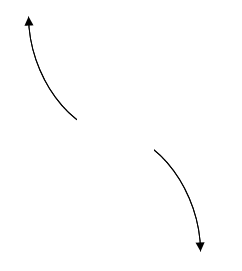
\includegraphics[width = 0.3\textwidth]{../Figures/polyEndBehaviorCopyAA.png}\item 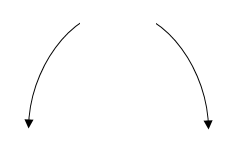
\includegraphics[width = 0.3\textwidth]{../Figures/polyEndBehaviorCopyBA.png}\item 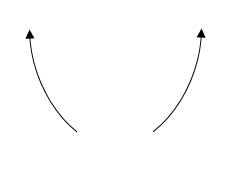
\includegraphics[width = 0.3\textwidth]{../Figures/polyEndBehaviorCopyCA.png}\item 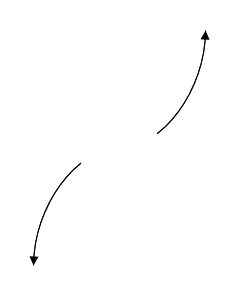
\includegraphics[width = 0.3\textwidth]{../Figures/polyEndBehaviorCopyDA.png}\end{multicols}\item None of the above.
\end{enumerate} }
\litem{
Describe the zero behavior of the zero $x = 3$ of the polynomial below.\[ f(x) = 6(x - 3)^{8}(x + 3)^{13}(x - 4)^{9}(x + 4)^{12} \]\begin{enumerate}[label=\Alph*.]
\begin{multicols}{2}\item 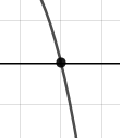
\includegraphics[width = 0.3\textwidth]{../Figures/polyZeroBehaviorAA.png}\item 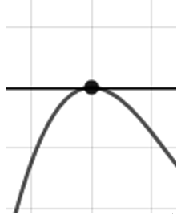
\includegraphics[width = 0.3\textwidth]{../Figures/polyZeroBehaviorBA.png}\item 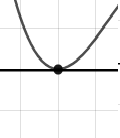
\includegraphics[width = 0.3\textwidth]{../Figures/polyZeroBehaviorCA.png}\item 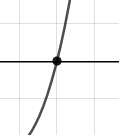
\includegraphics[width = 0.3\textwidth]{../Figures/polyZeroBehaviorDA.png}\end{multicols}\item None of the above.
\end{enumerate} }
\litem{
Which of the following equations \textit{could} be of the graph presented below?
\begin{center}
    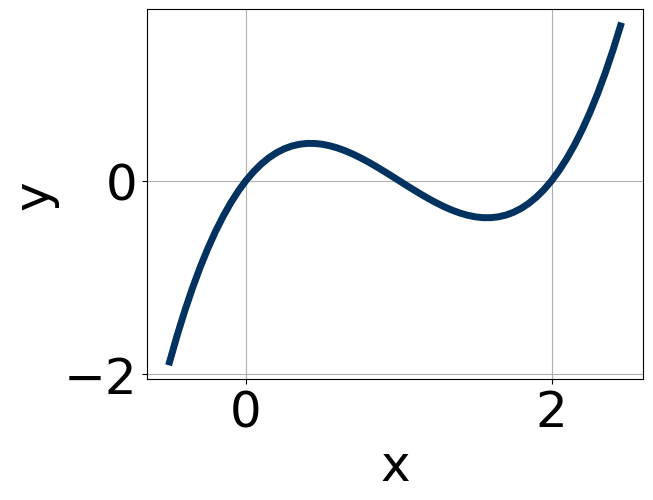
\includegraphics[width=0.5\textwidth]{../Figures/polyGraphToFunctionA.png}
\end{center}
\begin{enumerate}[label=\Alph*.]
\item \( 4x^{7} (x - 2)^{10} (x - 1)^{5} \)
\item \( -8x^{9} (x - 2)^{6} (x - 1)^{5} \)
\item \( 18x^{7} (x - 2)^{7} (x - 1)^{5} \)
\item \( 7x^{10} (x - 2)^{8} (x - 1)^{11} \)
\item \( -12x^{9} (x - 2)^{5} (x - 1)^{5} \)

\end{enumerate} }
\litem{
Construct the lowest-degree polynomial given the zeros below. Then, choose the intervals that contain the coefficients of the polynomial in the form $x^3+bx^2+cx+d$.\[ 4 + 5 i \text{ and } 2 \]\begin{enumerate}[label=\Alph*.]
\item \( b \in [7, 16], c \in [56, 57.3], \text{ and } d \in [81, 86.3] \)
\item \( b \in [0, 2], c \in [-6.8, -1.8], \text{ and } d \in [3.8, 8.5] \)
\item \( b \in [0, 2], c \in [-8.8, -6.5], \text{ and } d \in [8.4, 13.1] \)
\item \( b \in [-13, -4], c \in [56, 57.3], \text{ and } d \in [-84.9, -79.5] \)
\item \( \text{None of the above.} \)

\end{enumerate} }
\litem{
Which of the following equations \textit{could} be of the graph presented below?
\begin{center}
    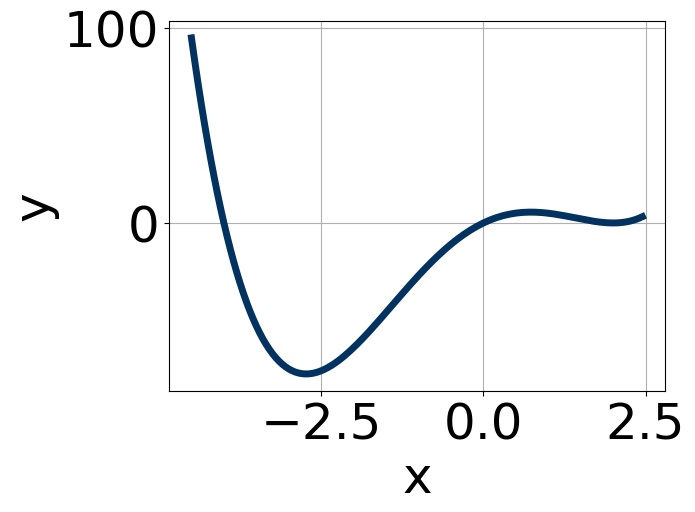
\includegraphics[width=0.5\textwidth]{../Figures/polyGraphToFunctionCopyA.png}
\end{center}
\begin{enumerate}[label=\Alph*.]
\item \( -18x^{9} (x - 2)^{10} (x + 4)^{8} \)
\item \( 19x^{6} (x - 2)^{9} (x + 4)^{9} \)
\item \( -14x^{9} (x - 2)^{6} (x + 4)^{5} \)
\item \( 11x^{9} (x - 2)^{8} (x + 4)^{7} \)
\item \( 19x^{6} (x - 2)^{10} (x + 4)^{9} \)

\end{enumerate} }
\litem{
Describe the end behavior of the polynomial below.\[ f(x) = -3(x + 2)^{3}(x - 2)^{8}(x + 6)^{5}(x - 6)^{5} \]\begin{enumerate}[label=\Alph*.]
\begin{multicols}{2}\item 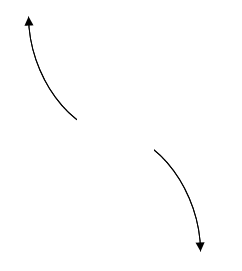
\includegraphics[width = 0.3\textwidth]{../Figures/polyEndBehaviorAA.png}\item 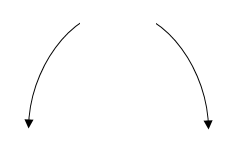
\includegraphics[width = 0.3\textwidth]{../Figures/polyEndBehaviorBA.png}\item 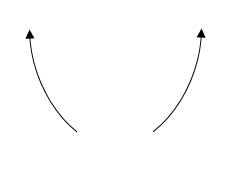
\includegraphics[width = 0.3\textwidth]{../Figures/polyEndBehaviorCA.png}\item 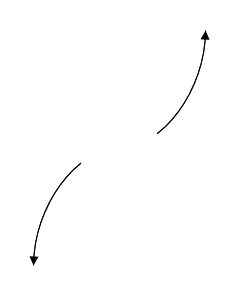
\includegraphics[width = 0.3\textwidth]{../Figures/polyEndBehaviorDA.png}\end{multicols}\item None of the above.
\end{enumerate} }
\litem{
Describe the zero behavior of the zero $x = 7$ of the polynomial below.\[ f(x) = 9(x + 8)^{9}(x - 8)^{7}(x - 7)^{7}(x + 7)^{2} \]\begin{enumerate}[label=\Alph*.]
\begin{multicols}{2}\item 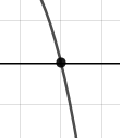
\includegraphics[width = 0.3\textwidth]{../Figures/polyZeroBehaviorCopyAA.png}\item 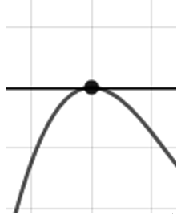
\includegraphics[width = 0.3\textwidth]{../Figures/polyZeroBehaviorCopyBA.png}\item 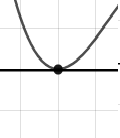
\includegraphics[width = 0.3\textwidth]{../Figures/polyZeroBehaviorCopyCA.png}\item 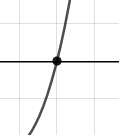
\includegraphics[width = 0.3\textwidth]{../Figures/polyZeroBehaviorCopyDA.png}\end{multicols}\item None of the above.
\end{enumerate} }
\litem{
Construct the lowest-degree polynomial given the zeros below. Then, choose the intervals that contain the coefficients of the polynomial in the form $ax^3+bx^2+cx+d$.\[ \frac{-1}{5}, \frac{-1}{4}, \text{ and } 6 \]\begin{enumerate}[label=\Alph*.]
\item \( a \in [16, 21], b \in [107, 116], c \in [-55, -47], \text{ and } d \in [-2, 13] \)
\item \( a \in [16, 21], b \in [-137, -123], c \in [51, 61], \text{ and } d \in [-9, -5] \)
\item \( a \in [16, 21], b \in [-113, -106], c \in [-55, -47], \text{ and } d \in [-2, 13] \)
\item \( a \in [16, 21], b \in [-120, -116], c \in [-19, -4], \text{ and } d \in [-2, 13] \)
\item \( a \in [16, 21], b \in [-113, -106], c \in [-55, -47], \text{ and } d \in [-9, -5] \)

\end{enumerate} }
\litem{
Construct the lowest-degree polynomial given the zeros below. Then, choose the intervals that contain the coefficients of the polynomial in the form $x^3+bx^2+cx+d$.\[ -5 + 4 i \text{ and } -2 \]\begin{enumerate}[label=\Alph*.]
\item \( b \in [-14, -10], c \in [53, 67], \text{ and } d \in [-88, -77] \)
\item \( b \in [1, 6], c \in [-5, -1], \text{ and } d \in [-8, 0] \)
\item \( b \in [1, 6], c \in [7, 8], \text{ and } d \in [9, 17] \)
\item \( b \in [9, 25], c \in [53, 67], \text{ and } d \in [82, 90] \)
\item \( \text{None of the above.} \)

\end{enumerate} }
\litem{
Construct the lowest-degree polynomial given the zeros below. Then, choose the intervals that contain the coefficients of the polynomial in the form $ax^3+bx^2+cx+d$.\[ \frac{-5}{4}, \frac{-3}{4}, \text{ and } -5 \]\begin{enumerate}[label=\Alph*.]
\item \( a \in [12, 18], b \in [44, 51], c \in [-145, -143], \text{ and } d \in [73, 83] \)
\item \( a \in [12, 18], b \in [104, 114], c \in [171, 181], \text{ and } d \in [-76, -74] \)
\item \( a \in [12, 18], b \in [72, 73], c \in [-60, -50], \text{ and } d \in [-76, -74] \)
\item \( a \in [12, 18], b \in [-114, -109], c \in [171, 181], \text{ and } d \in [-76, -74] \)
\item \( a \in [12, 18], b \in [104, 114], c \in [171, 181], \text{ and } d \in [73, 83] \)

\end{enumerate} }
\end{enumerate}

\end{document}